\fancyhead[C]{Sections 14.3-14.8, 15.1-15.4}
	\fancyhead[R]{HP Review Session}

\iftoggle{questions}{
\begin{center}{\large \textbf{Math 2551 HP Exam 2 Review}}
\end{center}


\begin{enumerate}
	
	
	\item Choose whether each statement is true or false. If the statement is 
	\textit{always} true, pick true. If the statement is \textit{ever} false, 
	pick false.  Give a reason for your answer.
		\begin{enumerate}
			\item If $f_x=f_y$ everywhere, then $f(x,y)$ is constant.
			
			\item There exists a function $f(x,y)$ with $f_x=2x+y$ and 
			$f_y=2x+2y$.
			
			\item If the temperature at a point $(x,y)$ on the floor of a room 
			is given by $T(x,y)$ and heat is being radiated out from a hot spot 
			at the origin, then if $a,b>0$ $\nabla T(a,b)$ could be $\langle 
			2,-2\rangle$.
			
			\item The integral $\iint_R y\ dA$ over the region $R: -1\leq x 
			\leq 1, 0\leq y \leq 1$ is zero.
		\end{enumerate}
	
	\item Based on the contour plot below, determine the signs of the requested 
	derivatives and draw the requested gradients.
	
	\begin{minipage}{0.45\textwidth}
		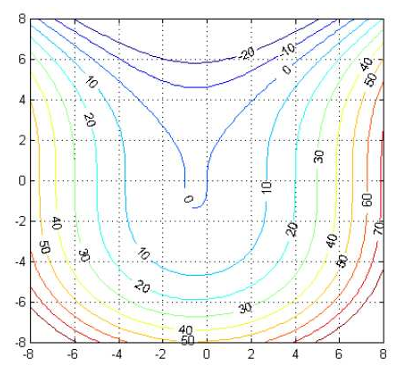
\includegraphics[scale=0.7]{hp_review_contour.png}
	\end{minipage}\begin{minipage}{0.45\textwidth}
	\begin{enumerate}
		\item $f_x(0,0)$ and $f_y(0,0)$
		\item $Df_{\bu}(2,-6)$, $u=\langle1/\sqrt{2},-1/\sqrt{2}\rangle$
		\item $\nabla f(-4,-4)$
		\item The rate of change of $f$ at $(-4,5)$ in the direction towards 
		$(4,6)$
	\end{enumerate}
	\end{minipage}
	
	\item Use the Chain Rule to find the total derivative of the composite 
	function $h=g\circ f$ at the point $(s,t)=(1,1)$, where \[ 
	f(s,t)=\begin{bmatrix}
		s^2+2t \\ 2s-t
	\end{bmatrix}\qquad g(x,y)=3x^2+4y^2.\]
	
	\item Which of the following gaurantees a saddle point of a continuously 
	differentiable function $f(x,y)$ at $(a,b)$?
	\begin{enumerate}
		\item $f_{xx}$ and $f_{yy}$ have the same sign at $(a,b)$
		\item $f_{xx}$ and $f_{yy}$ have opposite signs at $(a,b)$
		\item $f_{xy}$ is negative at $(a,b)$
		\item None of the above.
	\end{enumerate}
	
	\item Find and classify the critical points of $xy-2x-2y-x^2-y^2$. 
	
	\item Find the extreme values of $f(x,y,z)=2x+2y+z$ subject to the 
	constraint $x^2+y^2+z^2=9$. Interpret your results geometrically.
	
	\item Sketch the region of integration, set up iterated integrals for both 
	orders of integration, then evaluate using the easier order and explain why 
	it is easier. \[\iint_R y^2 e^{xy}\ dA, \quad R: x\geq 0, x\leq y \leq 4.\]
\end{enumerate}
}{}

\iftoggle{answers}{
\begin{center}{\large \textbf{Math 2551 HP Exam 2 Review Answers}}
\end{center}

\begin{enumerate}
	
	\item All are true except b).
	
	
	\item -1
	
	\item $\pm 1$
	
	\item Saddle at $(0,0)$ with $f(0,0)=0$, local min at $(0,2)$ of $-4$, local max at $(-2,0)$ of 4, saddle at $(-2,2)$ with $f(-2,2)=0$
	
	\item $(-1/2, 1/2, 1/2)$ and $(0,1,0)$
		
	\item $\sin(4)$
	
	\item No, this is less than $f(x,y)$ at all points, so it cannot possibly be the average value.
	
	\item $1800\pi$ cubic feet
\end{enumerate}
}{}
\iftoggle{solutions}
{
Solutions go here in the same format.
}{}
